\chapter{Architecture}

\section{Bobox}

In the section we describe basic architecture of Bobox. Information source for this chapter is Doctoral thesis Parallel Processing of Data\cite{faltthesis}. 

Overall Bobox architecture is displayed in figure~\ref{fig:bobox}. Framework contains of Boxes. Box is basically a C++ class containing implementation of data processing algorithm. Box can have arbitrary number of inputs and outputs. All boxes are connected to a directed acyclic graph.  

\begin{figure}[h!]
  \centering

    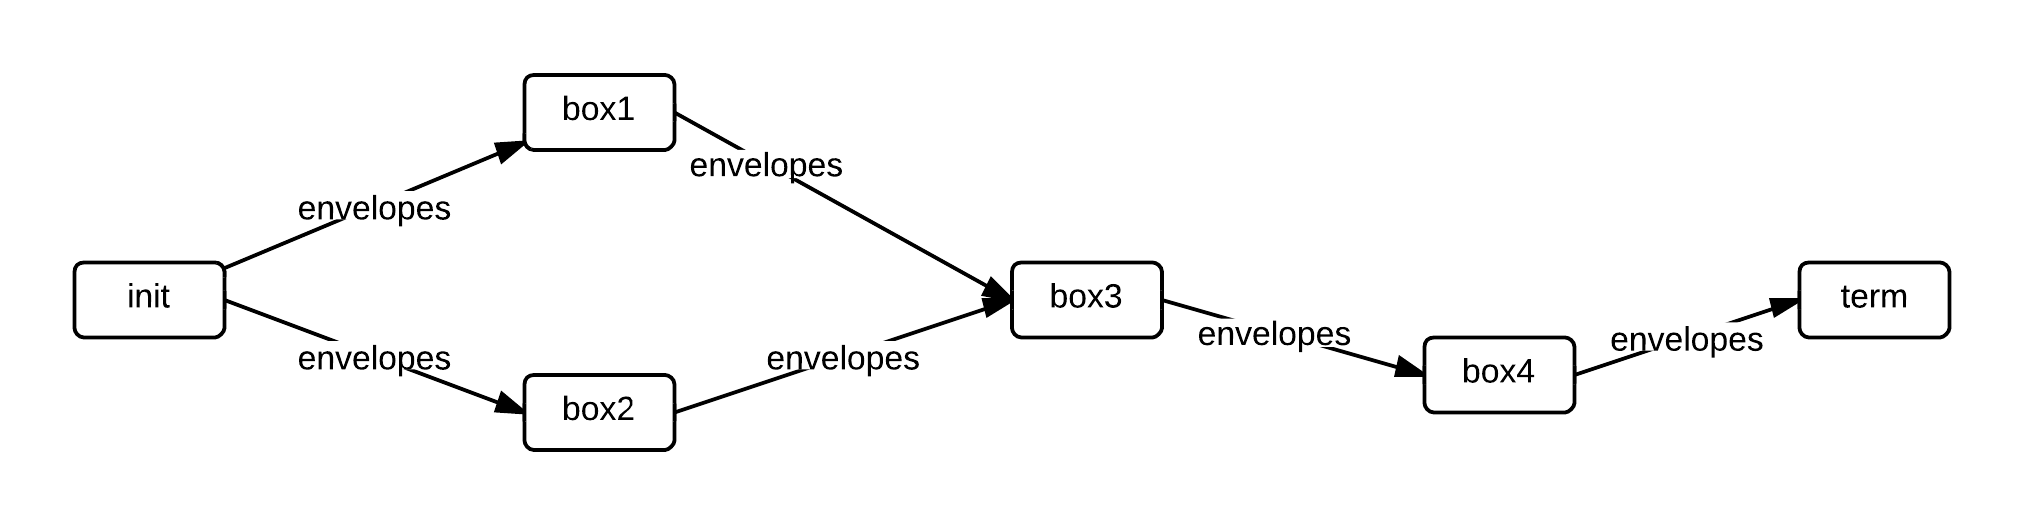
\includegraphics[width=1\textwidth]{bobox}
    
      \caption{Bobox architecture.}
        \label{fig:bobox}
\end{figure}

Data streams are implemented as data units called enveloped. Envelope structure is displayed in figure~\ref{fig:envelope}. It consists of sequence tuples, but internally data are stored by columns, that means envelope contains from sequence of columns and it's data is stored in separate list. So to read all attributes of the i-th tuple we have to access all column lists and read it's i-th element. There is special type of envelope having poisoned pill. It is send after all valid data indicating end of data stream. 

\begin{figure}[h!]
  \centering
    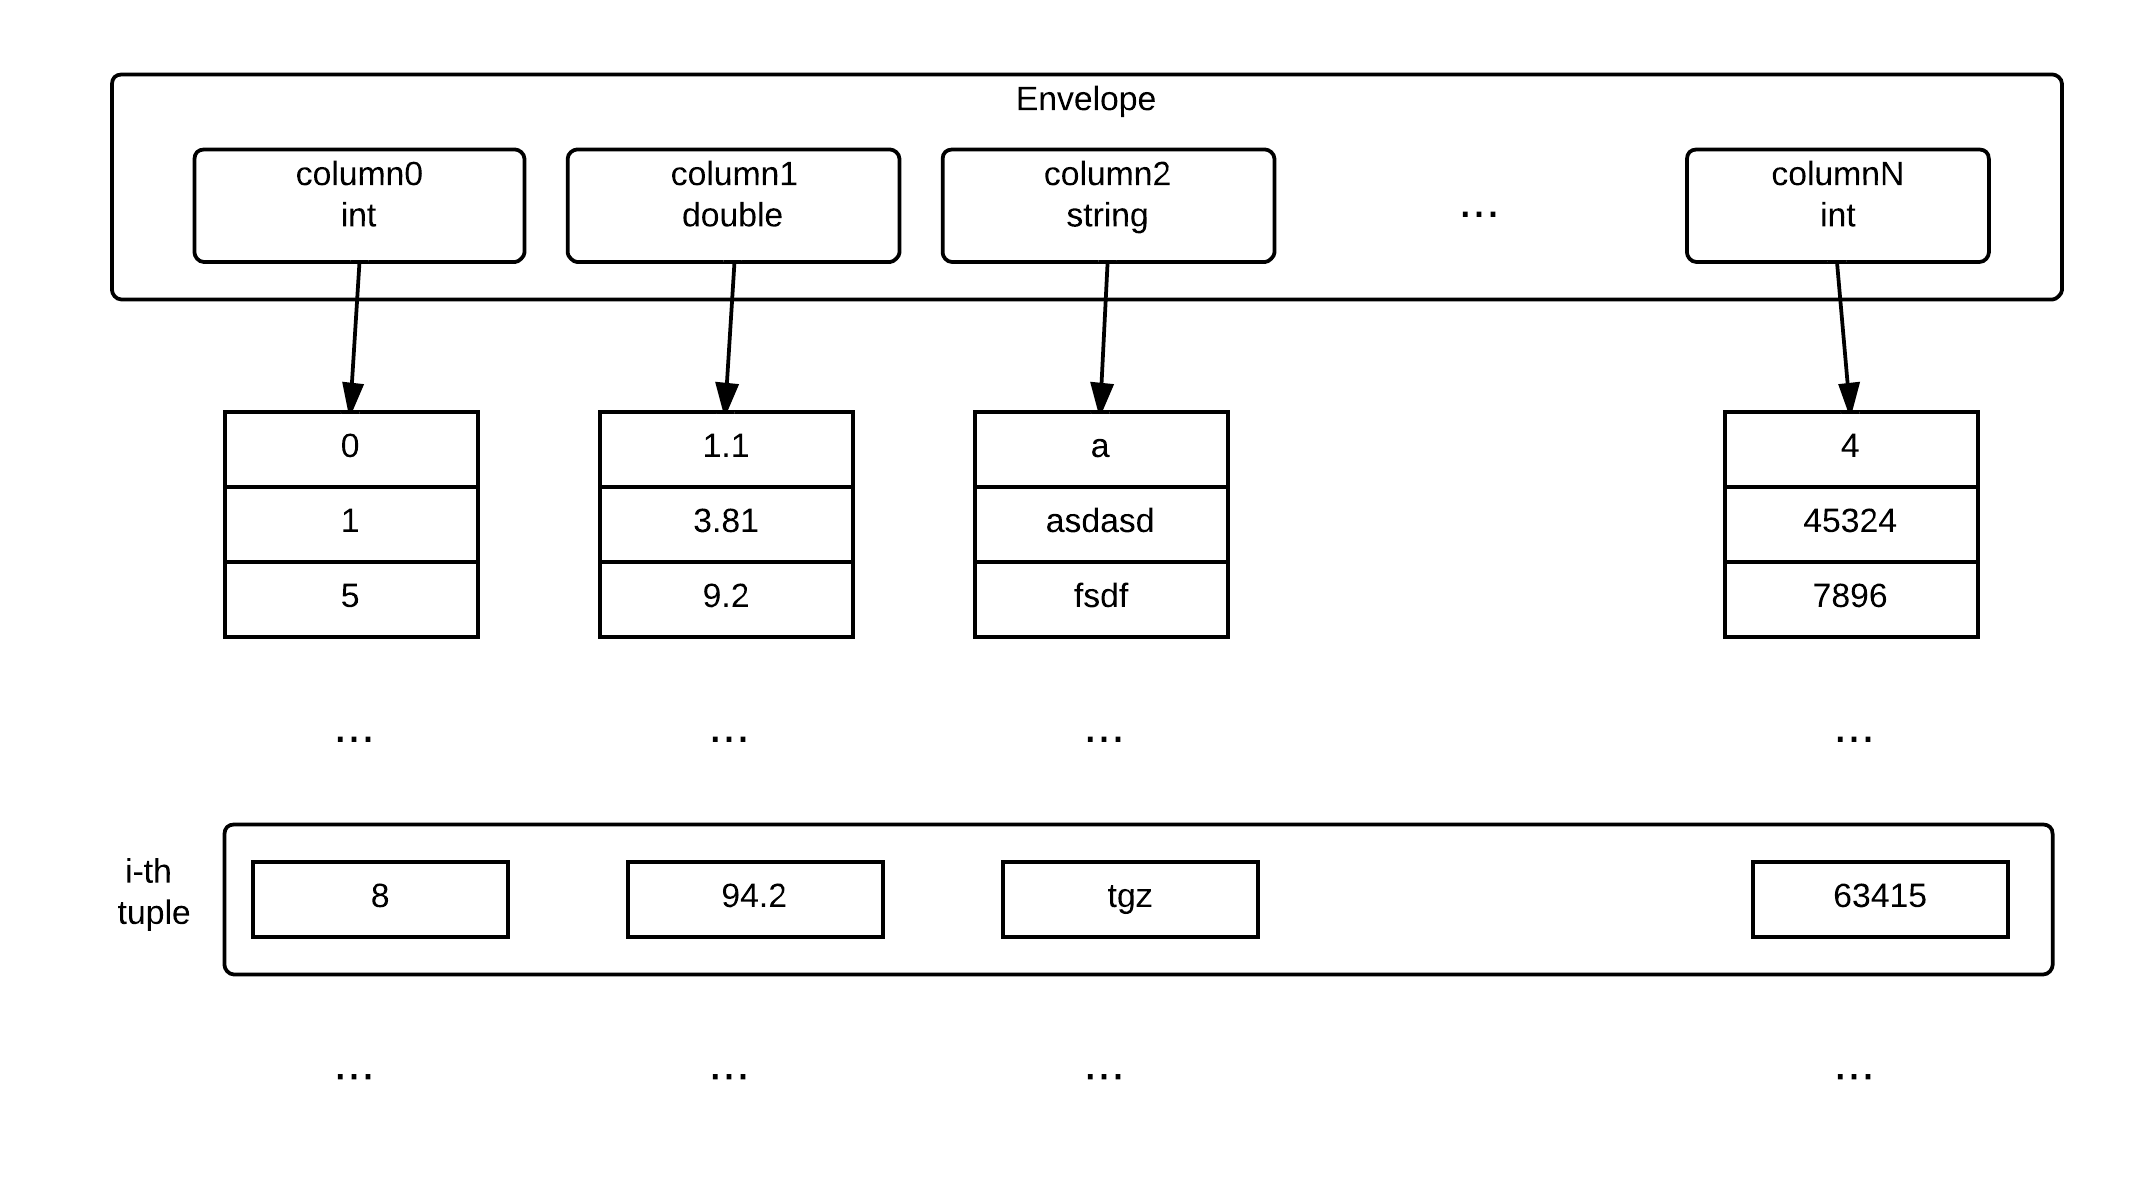
\includegraphics[width=1\textwidth]{envelope}

      \caption{Envelope structure.}
          \label{fig:envelope}
\end{figure}
There are two special boxes, which have to be in every execution plan:
\begin{itemize}


\item $init$ - first box in topological order and it indicates starting box of execution plan

\item $term$ - last box in topological order and indicates that plan has been completely evaluated

\end{itemize}

Evaluation starts with scheduling $init$ box, which sends poisoned pills to all of its output. All of it's output boxes will be scheduled. They can read data from hard drive or network, process it and sent it to other boxes for further processing. Other boxes usually receives data in envelopes in their inputs. Box $term$ waits for every it's input to receive poisoned pill and then evaluation ends.

\section{Bobolang}

\section{Architecture}

\section{Goal}